\documentclass[conference]{IEEEtran}
\IEEEoverridecommandlockouts
% The preceding line is only needed to identify funding in the first footnote. If that is unneeded, please comment it out.
\usepackage{cite}
\usepackage{amsmath,amssymb,amsfonts}
\usepackage{algorithmic}
\usepackage{graphicx}
\usepackage{textcomp}
\usepackage{xcolor}
\usepackage{enumitem}
\def\BibTeX{{\rm B\kern-.05em{\sc i\kern-.025em b}\kern-.08em
    T\kern-.1667em\lower.7ex\hbox{E}\kern-.125emX}}
\begin{document}

\title{AIMI Group 19, Panorama\\
% {\footnotesize \textsuperscript{*}Note: Sub-titles are not captured in Xplore and
% should not be used}
\thanks{Identify applicable funding agency here. If none, delete this.}
}

\author{\IEEEauthorblockN{1\textsuperscript{st} Giedrius Mirklys}
\IEEEauthorblockA{\textit{Faculty of Science} \\
\textit{Radboud University}\\
Nijmegen, Netherlands \\
giedrius.mirklys@ru.nl}
\and
\IEEEauthorblockN{2\textsuperscript{nd} Ignas Golubovskis}
\IEEEauthorblockA{\textit{Faculty of Science} \\
\textit{Radboud University}\\
Nijmegen, Netherlands \\
ignas.golubovskis@ru.nl}
\and
\IEEEauthorblockN{3\textsuperscript{rd} Björn Westerlund}
\IEEEauthorblockA{\textit{Faculty of Science} \\
\textit{Radboud University}\\
Nijmegen, Netherlands \\
bjoern.westerlund@ru.nl}
\and
\IEEEauthorblockN{4\textsuperscript{th} Luka Godnič}
\IEEEauthorblockA{\textit{Faculty of Science} \\
\textit{Radboud University}\\
Nijmegen, Netherlands \\
luka.godnic@ru.nl}
}

\maketitle

\begin{abstract}
Pancreatic ductal adenocarcinoma (PDAC) is among the deadliest malignancies, often eluding early detection due to its subtle presentation on contrast-enhanced CT (CECT) scans. The PANORAMA challenge provides a large-scale, multi-reader benchmark for PDAC detection, offering a unique opportunity to evaluate and enhance machine-learning–based diagnostic tools. In this project, we aimed to improve upon the winning submission of the PANORAMA competition, which leverages the nnU-Net framework for segmentation and classification. Our focus was on reducing false positives to minimize radiologist workload, primarily by incorporating the Tversky loss function, which allows fine-tuning the trade-off between false positives and false negatives. We analyzed the effect of this modification on detection accuracy and the area under the ROC curve (AUC), and further evaluated segmentation performance using Dice score metrics. This report details our methodological improvements, experimental results, and future directions for robust, generalizable PDAC detection models.

\end{abstract}

\section{Introduction}
As part of course Artificial Inteligence in Medical Imaging (AIMI)\cite{b4}, we were tasked with improving the baseline model of \textsc{PANORAMA}\cite{b5} challenge. The PANORAMA challenge is the first large-scale reader study which aimed to establish the baseline performance of radiologists at Pancreatic Ductal Adenocarcinoma (PDAC)(add reference) detection on CECT scans. PDAC) is the most common type of malignant tumor affecting the pancreas and ranks among the deadliest of all solid cancers. In the United States, it is projected that there will be approximately 67,440 new cases and 51,980 deaths from PDAC in 2025\cite{b2}.
% \begin{figure}
%     \centering
%     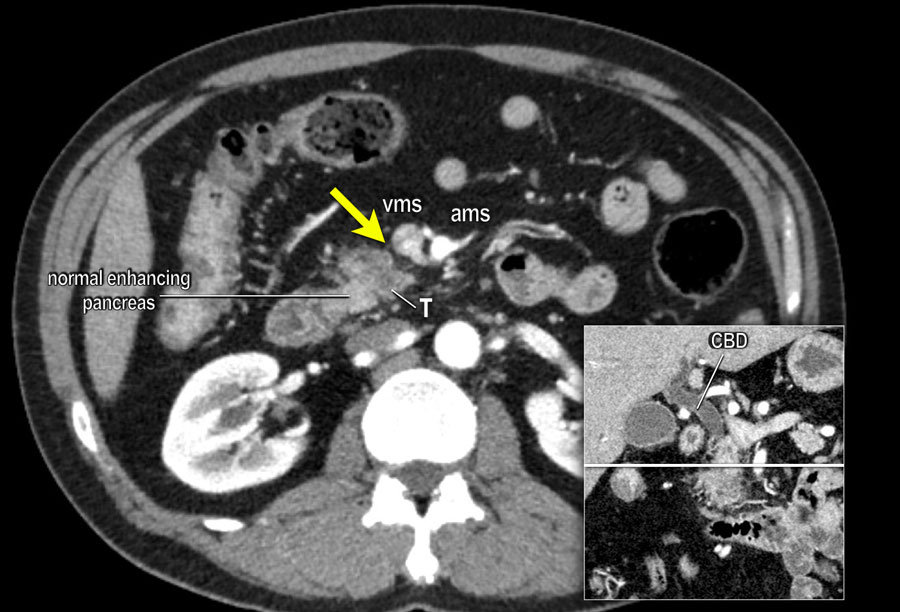
\includegraphics[width=0.75\linewidth]{pancreatic_cancer.jpg}
%     \caption{Part of a CT scan showing a patient with pancreatic cancer\cite{b6}}
%     \label{fig:ct_scan}
% \end{figure}
The challenge included more  68 international readers and more than 400 cases in the hidden testing cohort. Readers study was two fold. The first task was giving a discrete diagnosis with an additional PDAC likelihood score, and the second task readers provided a point annotation of the leasion location in the PDAC cases.

\section{Related work}
\section{Motivation for Machine-Learning–Driven PDAC Detection}
Pancreatic ductal adenocarcinoma (PDAC) often leaves only faint radiologic footprints—e.g.\ minimal ductal calibre changes or subtle parenchymal texture shifts—on contrast-enhanced CT (CECT) months before a tumour becomes obvious.  These patterns are easily missed by experts reviewing thousands of abdominal scans for diverse indications.  Modern deep-learning systems, however, thrive on precisely this kind of weak-signal problem: by optimising millions of parameters across 3-D feature hierarchies, they can amplify and aggregate minute cues that fall below human perceptual thresholds \cite{b7, b8}.

The \textsc{Panorama} grand challenge provides the first large-scale test bed for such systems in PDAC, with the following distinguishing characteristics:  
\begin{itemize}[leftmargin=*]
  \item \textbf{Data volume.}  Annotated scans of $>$2\,500 cases for open development.
  \item \textbf{Human baseline.} 68 international radiologists supply a reader-study benchmark, enabling rigorous algorithm-vs-expert comparison.
  \item \textbf{Task design.}  Algorithms are evaluated on (i) binary PDAC presence scores and (ii) voxel-level lesion localisation, mirroring real-world deployment needs.
\end{itemize}

State-of-the-art deep learning approaches, such as the PANDA model described by Cao et al. (2023) which utilizes components like CNNs and transformers, have reported NCCT AUCs $>0.95$ for pancreatic lesion detection on single-centre cohorts.\cite{b9}. Yet external validation is rare, and most models are tuned on datasets an order of magnitude smaller than \textsc{Panorama}. Critically, these smaller datasets typically have fewer different data sources, leading to lower overall variance between samples, which will likely boost prediction scores but is unlikely to generalize well.

\subsection{Model starting point}
We chose to use the winning submission of the PANORAMA competition as starting point for out own experiments. We considered using the competition baseline but found them to be very similar, with the competition winner's repo being easier to follow. This approach uses nnUnet \cite{b1} an out of the box neural net solution that builds on the U-net architecture that is specifically tuned for biomedical use cases and contains. Additionally, it can automatically adapt preprocessing, neural net architecture, and post processing according to the data it is classifying.

The full inference pipeline consists of 4 steps: down-sampling, low-res prediction, masking and high-res prediction. First images are loaded and the voxels are down-sampled according to a set spacing, main to save. Then the nnU-net makes a mask prediction, aiming to identify the rough area of the pancreas. This is very important as the pancreas is quite small and the CECT scans used as input cover the whole body of the patients. Standardized down-sampling is important in order to save computational cost without losing predictive ability. The mask is represented as a bounding box and in the next step, this bounding box is applied to the original image. Then a second prediction is made, this time at full resolution but only using the area within the bounding box. This prediction produces two outputs, the full scan of the patient with lesion candidate likelihoods applied to each voxel as well as a single number representing the probability that a patient has a pancreatic lesion.

\[
\text{TI} = \frac{\text{TP}}{\text{TP} + \alpha \cdot \text{FN} + \beta \cdot \text{FP}}
\]


\section{Improving the baseline}
When considering how to improve the baseline, we explored various potential approaches and evaluated their feasibility. We quickly determined that the most effective objective was to shift the AUC curve to the left. This shift reduces the false positive (FP) rate, thereby decreasing the workload for radiologists and physicians, who must review all cases flagged as positive.

One of the approaches we explored was training the network using the Tversky loss, a loss function commonly used in medical image analysis. It measures the dissimilarity between two sets—typically the predicted segmentation and the ground truth—and is a generalization of the Jaccard index.\cite{b3} By tuning the parameters $\alpha$ and $\beta$, you can control how the loss penalizes different types of segmentation errors. For instance, setting $\alpha$ $>$ $\beta$ places greater emphasis on reducing false positives, whereas $\beta$ $>$ $\alpha$ focuses more on minimizing false negatives. This flexibility allows Tversky loss to fine-tune the trade-off between precision and recall, making it particularly useful in scenarios where the cost of false positives and false negatives is not equal. In our case, where minimizing false positives and maximizing precision is crucial, Tversky loss provides an effective way to bias the model accordingly.

There are a few more things we need to describe in the report: 

- checking the data: balance and differences in test and training data
- besides the loss, dice score curves of both baseline and tversky, maybe some outputs of the filters

- some FP/FN analysis.


\section{Results}
TODO
\section{Conclusions}
TODO

This document is a model and instructions for \LaTeX.
This and the IEEEtran.cls file define the components of your paper [title, text, heads, etc.]. *CRITICAL: Do Not Use Symbols, Special Characters, Footnotes, 
or Math in Paper Title or Abstract.

\begin{IEEEkeywords}
component, formatting, style, styling, insert
\end{IEEEkeywords}

\begin{thebibliography}{00}
\bibitem{b1} Isensee, F., Jaeger, P.F., Kohl, S.A.A. et al. nnU-Net: a self-configuring method for deep learning-based biomedical image segmentation. Nat Methods 18, 203–211 (2021). https://doi.org/10.1038/s41592-020-01008-z
\bibitem{b2} National Cancer Institute, ``SEER Cancer Stat Facts: Pancreatic Cancer,'' https://seer.cancer.gov/statfacts/html/pancreas.html, accessed May 15, 2025.
\bibitem{b3} Saba, M., ``Tversky Loss,'' *Medium*, https://medium.com/@saba99/tversky-loss-902f5f8cc35f, accessed May 15, 2025.
\bibitem{b4} Radboud University, ``Course: NWI-IMC037 – Artificial Intelligence and Medical Imaging,'' Osiris Course Catalogue, https://ru.osiris-student.nl/onderwijscatalogus/extern/cursus?taal=en\&cursuscode=NWI-IMC037\&collegejaar=2024, accessed May 15, 2025.
\bibitem{b5} PANORAMA Grand Challenge, ``PANORAMA: AI Grand Challenge for Pancreatic Cancer Detection,'' https://panorama.grand-challenge.org/, accessed May 15, 2025.
\bibitem{b6} The Radiology Assistant, ``Pancreas - Carcinoma,'' https://radiologyassistant.nl/abdomen/pancreas/pancreas-carcinoma-1, accessed May 15, 2025.
\bibitem{b7} A. Esteva, B. Kuprel, R. A. Novoa, J. Ko, S. M. Swetter, H. M. Blau, and S. Thrun, ``Dermatologist-level classification of skin cancer with deep neural networks,'' \textit{Nature}, vol. 542, no. 7639, pp. 115--118, 2017, doi: 10.1038/nature21056.
\bibitem{b8} S. M. McKinney, M. Sieniek, V. Godbole, J. Godwin, N. Antropova, H. Ashrafian, T. Back, A. Chesus, D. C. Corrado, B. Darzi, \textit{et al.}, ``International evaluation of an AI system for breast cancer screening,'' \textit{Nature}, vol. 577, no. 7788, pp. 89--94, 2020, doi: 10.1038/s41586-019-1799-6.
\bibitem{b9} K. Cao, Y. Xia, J. Yao, H. Xu, L. Lambert, T. Zhang, W. Tang, G. Jin, J. Hui, F. Xu, I. Nogues, X. Li, W. Guo, Y. Wang, W. Fang, M. Qiu, Y. Hou, T. Kovarnik, M. Vocka, Y. Lu, Y. Chen, X. Chen, Z. Liu, Z. Chen, C. Xie, R. Zhang, H. Lu, G. Hager, A. L. Yuille, L. Lu, C. Shao, Y. Shi, T. Liang, L. Zhang, and J. Lu, ``Large-scale pancreatic cancer detection via non-contrast CT and deep learning,'' \textit{Nature Medicine}, vol. 29, no. 12, pp. 3033--3043, 2023, doi: 10.1038/s41591-023-02640-w.







\end{thebibliography}
\end{document}
